\documentclass[11pt]{amsart}
\usepackage{amsmath,amssymb,amsthm}
\usepackage{graphicx}
\usepackage[hidelinks]{hyperref}

\newtheorem{theorem}{Theorem}
\newtheorem{lemma}{Lemma}
\newtheorem{corollary}{Corollary}
\newtheorem{remark}{Remark}

\newcommand{\R}{\mathbb R}
\newcommand{\Hh}{\mathbb H}
\newcommand{\ellinf}{\ell^\infty}
\newcommand{\Lip}{\operatorname{Lip}}
\newcommand{\Repart}{\operatorname{Re}}

\title[Heisenberg horizontal-line embedding]{A horizontal-line embedding answer for Wildrick's Heisenberg Bochner-derivative questions}
\author{fa\_banach\_001, agent\_super\_00}
\date{2026-07-01}

\begin{document}
\maketitle

\section*{Status}

This packet gives affirmative answers to Problems 5.3, 5.4, and 5.5 in
Wildrick \cite{Wildrick}.  The key point is that the sub-Riemannian Heisenberg
group has a 1-Lipschitz retraction onto any chosen horizontal line.  Combining
that retraction with a Kuratowski embedding gives a Banach-space embedding that
is exactly linear on the chosen line.

\section*{Source questions}

The relevant source passage is on PDF page 5.  Problem 5.3 asks whether, for
the Heisenberg group, there is any nonconstant map into $\Hh$ and any
bi-Lipschitz embedding into a Banach space for which the Bochner partial
derivatives exist.  Problem 5.4 asks whether some embedding has a nonzero
velocity at some point.  Problem 5.5 asks the simpler concrete version:
whether there is a bi-Lipschitz embedding $\iota:\Hh\to V$ and a vector
$\vec v\in V$ such that
\[
 \iota(x+0i,0)=x\vec v
 \qquad (x\in\R).
\]

\begin{center}
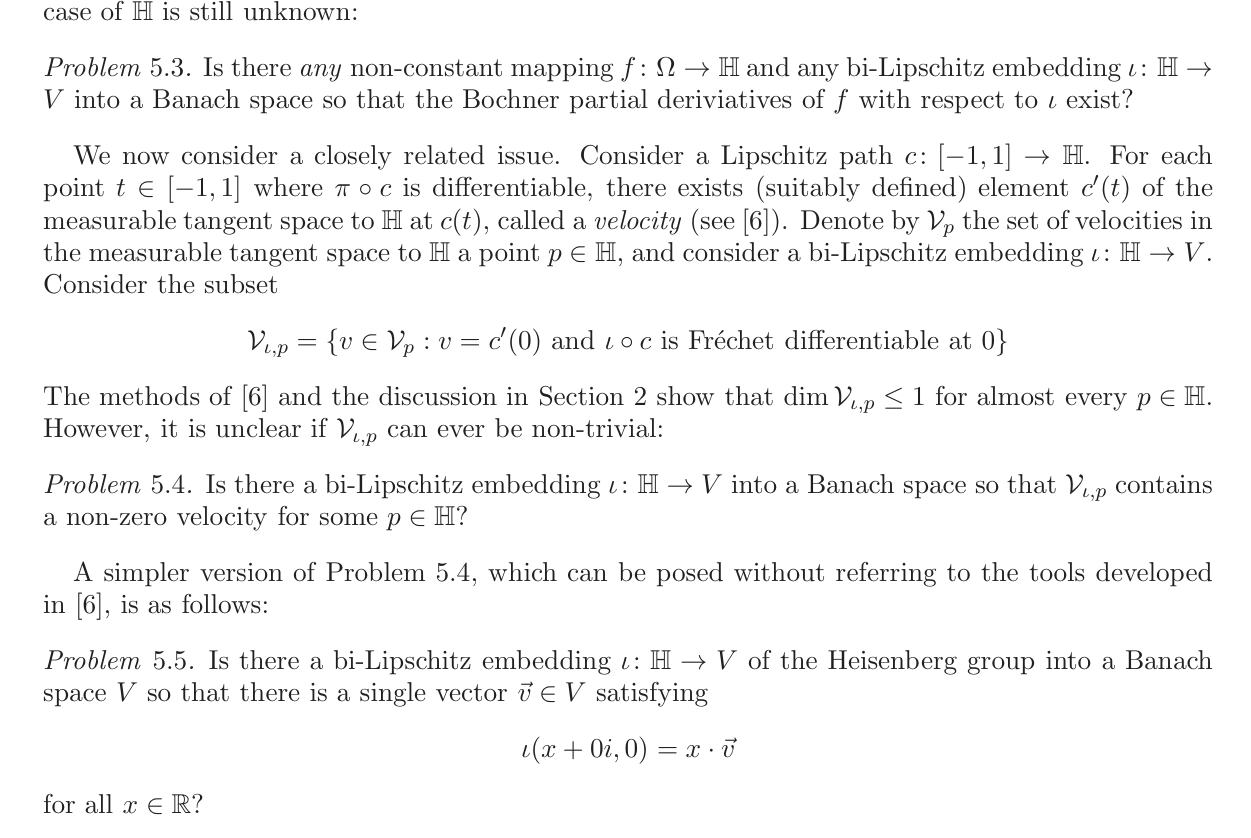
\includegraphics[width=0.96\textwidth]{figures/problems_5_3_to_5_5_crop.png}
\end{center}

\section*{Proof Intuition}

A Kuratowski embedding remembers all distances, but it has no reason to be
linear on a selected geodesic.  If the selected geodesic is the range of a
1-Lipschitz retraction $r$, we can keep the linear coordinate on the geodesic
and use the difference
\[
 \kappa(x)-\kappa(r(x))
\]
for the remaining coordinates.  This difference vanishes on the geodesic.  It
still controls the lost metric information because
\[
 \kappa(x)-\kappa(y)
 =
 \bigl(\kappa(x)-\kappa(r(x))\bigr)
 -
 \bigl(\kappa(y)-\kappa(r(y))\bigr)
 +
 \bigl(\kappa(r(x))-\kappa(r(y))\bigr).
\]
Thus the original distance is bounded by the new transverse part plus the
linear retraction coordinate.

\section*{A retract lemma}

\begin{lemma}
\label{lem:retract}
Let $(X,d)$ be a separable metric space.  Suppose that
$\ell:\R\to X$ is an isometric embedding and that $r:X\to \ell(\R)$ is a
1-Lipschitz retraction.  Write $a:X\to\R$ for the coordinate defined by
$r(x)=\ell(a(x))$.  Then there is a Banach space $V$ and a bi-Lipschitz
embedding $I:X\to V$ such that
\[
 I(\ell(s))=s v
 \qquad (s\in\R)
\]
for a nonzero vector $v\in V$.
\end{lemma}

\begin{proof}
Let $\kappa:X\to\ellinf$ be any Kuratowski isometric embedding.  Set
\[
 V=\R\oplus_\infty \ellinf
\]
and define
\[
 I(x)=\bigl(a(x),\,\kappa(x)-\kappa(r(x))\bigr).
\]
If $x=\ell(s)$, then $r(x)=x$ and $a(x)=s$, so
$I(\ell(s))=(s,0)=s(1,0)$.  Put $v=(1,0)$.

Since $r$ is 1-Lipschitz and $\ell$ is isometric, the coordinate $a$ is
1-Lipschitz.  The second component is 2-Lipschitz, because
\[
 \|\kappa(x)-\kappa(r(x))-\kappa(y)+\kappa(r(y))\|_\infty
 \le d(x,y)+d(r(x),r(y))
 \le 2d(x,y).
\]
Hence $I$ is 2-Lipschitz.

For the lower estimate, use that $\kappa$ is isometric:
\begin{align*}
 d(x,y)
 &=\|\kappa(x)-\kappa(y)\|_\infty\\
 &\le
 \|\kappa(x)-\kappa(r(x))-\kappa(y)+\kappa(r(y))\|_\infty
   +\|\kappa(r(x))-\kappa(r(y))\|_\infty\\
 &=
 \|\kappa(x)-\kappa(r(x))-\kappa(y)+\kappa(r(y))\|_\infty
   +|a(x)-a(y)|\\
 &\le 2\|I(x)-I(y)\|_V.
\end{align*}
Thus $\|I(x)-I(y)\|_V\ge d(x,y)/2$, and $I$ is bi-Lipschitz.
\end{proof}

\section*{Application to the Heisenberg group}

Let $\Hh$ be the first Heisenberg group with its standard CC metric $d_{cc}$.
Let
\[
 \ell(s)=(s+0i,0).
\]
This is an isometric copy of $\R$: the horizontal curve $s\mapsto (s+0i,0)$
has length equal to the Euclidean length, and every horizontal curve joining
$\ell(s)$ to $\ell(t)$ has length at least $|s-t|$ because its real horizontal
coordinate changes by $s-t$.

Define
\[
 r(z,t)=(\Repart z+0i,0).
\]
The same length estimate shows that $r$ is 1-Lipschitz, since
\[
 d_{cc}(r(z,t),r(w,u))=|\Repart z-\Repart w|\le d_{cc}((z,t),(w,u)).
\]
Therefore Lemma \ref{lem:retract} applies to $\Hh$.

\begin{theorem}
\label{thm:problem55}
There exists a Banach space $V$, a bi-Lipschitz embedding
$I:\Hh\to V$, and a nonzero vector $v\in V$ such that
\[
 I(x+0i,0)=xv
 \qquad (x\in\R).
\]
Thus Problem 5.5 of \cite{Wildrick} has an affirmative answer.
\end{theorem}

\begin{proof}
Apply Lemma \ref{lem:retract} to the horizontal line $\ell$ and the retraction
$r$ above.
\end{proof}

\section*{Consequences for Problems 5.3 and 5.4}

\begin{corollary}
Problem 5.4 of \cite{Wildrick} has an affirmative answer.
\end{corollary}

\begin{proof}
Let $I$ be the embedding in Theorem \ref{thm:problem55}.  For the horizontal
path $c(t)=(t+0i,0)$, one has $I(c(t))=tv$, so $I\circ c$ is Frechet
differentiable at $0$ with derivative $v\ne0$.  In the usual Cheeger
differentiable structure on $\Hh$, this path has the nonzero horizontal
velocity in the real direction at the identity.  Hence
$\mathcal V_{I,0}$ contains a nonzero velocity.
\end{proof}

\begin{corollary}
Problem 5.3 of \cite{Wildrick} has an affirmative answer.  In fact, for every
bounded Euclidean domain $\Omega\subset\R^n$ there is a nonconstant Lipschitz
map $f:\Omega\to\Hh$ and a bi-Lipschitz embedding $I:\Hh\to V$ such that the
Bochner partial derivatives of $I\circ f$ exist and are integrable.
\end{corollary}

\begin{proof}
Use the embedding $I$ from Theorem \ref{thm:problem55} and define
\[
 f(x_1,\ldots,x_n)=(x_1+0i,0).
\]
Then $f$ is Lipschitz and nonconstant on any Euclidean domain.  Moreover
\[
 I(f(x_1,\ldots,x_n))=x_1v.
\]
Thus $I\circ f$ has the constant Bochner partial derivative $v$ in the first
coordinate and zero Bochner partial derivatives in all other coordinates.
Since $\Omega$ is bounded, these derivatives are integrable.
\end{proof}

\section*{Scope and novelty}

This result answers only the Heisenberg existence questions 5.3, 5.4, and 5.5.
It does not characterize the Poincare-inequality spaces in Problem 5.1, and it
does not characterize the metric spaces with an $\iota$-Radon-Nikodym embedding
in Problem 5.2.  It also does not contradict the source's main theorem: the
construction gives one good family of maps along one horizontal line, while the
main theorem rules out embeddings that make every Lipschitz map into a Cheeger
fractal Bochner differentiable.

Before promotion, the cheap run indexes were searched for the arXiv id, the
source title, Bochner partial derivatives, Cheeger-Kleiner differentiability,
$\iota$-Radon-Nikodym terminology, nonzero velocity, and the exact
Problem 5.5 horizontal-line formula.  No duplicate packet or prior attempt was
found.  Local full-source fixed-string searches found only the source
questions themselves.  A bounded web search on 2026-07-01 for the exact
horizontal-line formula and the source title with ``single vector'' did not
surface a later answer.

\section*{Human review recommendation}

The proof is metric and should be checked mainly at one point: under the
standard Carnot-Caratheodory normalization, the coordinate retraction
$(z,t)\mapsto(\Repart z+0i,0)$ is 1-Lipschitz.  Once this is accepted, the
retract lemma gives the bi-Lipschitz embedding formally.

\begin{thebibliography}{2}

\bibitem{Heinonen}
J. Heinonen,
\emph{Lectures on analysis on metric spaces},
Universitext, Springer, 2001.

\bibitem{Wildrick}
K. Wildrick,
\emph{Bochner Partial Derivatives, Cheeger-Kleiner Differentiability, and
Non-Embedding},
arXiv:2307.10857, 2023.

\end{thebibliography}

\end{document}
